\documentclass[aspectratio=169,10pt]{beamer}
\usepackage{../common/beamer_theme_bio}

\title{\textbf{Biostatistiques Appliquées}}
\subtitle{Chapitre VI : Classification Hiérarchique Ascendante (CAH) \& Dendrogrammes}
\author{\textbf{Dr. Sarra BENMOUMOU (Ph.D.)}}
\institute{
  Faculté des Sciences --- Département de Biologie\\
  Master 2 : Biochimie Appliquée\\
  \textbf{Université M'Hamed Bougara de Boumerdès (UMBB)}
}
\date{Année Universitaire 2024 -- 2025}

\begin{document}

\begin{frame}[plain]
  \titlepage
\end{frame}

\begin{frame}{Plan Détaillé du Chapitre VI}
  \tableofcontents
\end{frame}

% ========================================================
\section{Objectifs de la CAH en Biologie}
% ========================================================

\begin{frame}{La Classification Non Supervisée}
  \begin{columns}[onlytextwidth, T]
    \begin{column}{0.48\linewidth}
      \begin{conceptbox}{Définition \& Philosophie}
        Contrairement aux modèles prédictifs guidés :
        \begin{itemize}
          \item Les groupes d'individus ou de biomolécules ne sont \textbf{pas connus à l'avance}.
          \item L'algorithme cherche à regrouper les entités les plus ressemblantes de manière ascendante (du bas vers le haut).
          \item Fournit une représentation sous forme d'arbre : le \textbf{Dendrogramme}.
        \end{itemize}
      \end{conceptbox}
    \end{column}
    \begin{column}{0.48\linewidth}
      \begin{biobox}{Applications Clés en Biochimie}
        \begin{itemize}
          \item \textbf{Microbiologie :} Sous-typage de souches bactériennes d'après leurs profils enzymatiques et antibiogrammes.
          \item \textbf{Oncologie Moléculaire :} Identification de nouveaux sous-types de cancers à partir de biomarqueurs protéiques.
          \item \textbf{Génomique :} Regroupement de gènes co-exprimés ou co-régulés.
        \end{itemize}
      \end{biobox}
    \end{column}
  \end{columns}
\end{frame}

% ========================================================
\section{Distances \& Critères d'Agrégation}
% ========================================================

\begin{frame}{1. Mesures de Dissimilarité Biologique}
  \begin{columns}[onlytextwidth, T]
    \begin{column}{0.48\linewidth}
      \begin{conceptbox}{Distance Euclidienne}
        \begin{equation*}
          d(x,y) = \sqrt{\sum_{k=1}^p (x_k - y_k)^2}
        \end{equation*}
        \begin{itemize}
          \item Mesure géométrique classique.
          \item Très sensible aux unités absolues (exige des données \textbf{préalablement centrées-réduites}).
        \end{itemize}
      \end{conceptbox}
    \end{column}
    \begin{column}{0.48\linewidth}
      \begin{conceptbox}{Distance de Corrélation}
        \begin{equation*}
          d_{\text{cor}}(x,y) = 1 - r(x,y)
        \end{equation*}
        \begin{itemize}
          \item Regroupe les protéines ou gènes ayant la \textbf{même cinétique temporelle}, même si l'amplitude basale est très différente.
          \item Essentielle pour l'analyse d'expression génique.
        \end{itemize}
      \end{conceptbox}
    \end{column}
  \end{columns}
\end{frame}

\begin{frame}{2. Critères d'Agrégation (Méthodes de Liaison)}
  \begin{table}[h]
    \centering
    \small
    \resizebox{\linewidth}{!}{%
    \begin{tabular}{lp{6cm}p{5.5cm}}
      \toprule
      \textbf{Méthode} & \textbf{Principe Mathématique de Fusion} & \textbf{Comportement Biologique} \\
      \midrule
      \textbf{Lien Simple} & Distance minimale entre deux éléments des groupes & Tendance fâcheuse au « chaînage » (regroupe les points isolés en filaments). \\
      \midrule
      \textbf{Lien Complet} & Distance maximale entre deux éléments & Forme des groupes très compacts et sphériques. \\
      \midrule
      \textbf{Lien Moyen (UPGMA)} & Moyenne arithmétique de toutes les distances croisées & Standard historique de la phylogénie moléculaire. \\
      \midrule
      \textbf{Méthode de Ward} & Fusionne les deux groupes qui minimisent la perte d'inertie intra-groupe ($\Delta I_{\text{intra}}$) & \cellcolor{BioGreen!20}\textbf{Recommandée en biochimie pour obtenir des groupes homogènes et équilibrés.} \\
      \bottomrule
    \end{tabular}%
    }
  \end{table}
\end{frame}

% ========================================================
\section{Le Dendrogramme \& Les Heatmaps}
% ========================================================

\begin{frame}{Lecture du Dendrogramme \& Seuil de Coupure}
  \begin{center}
    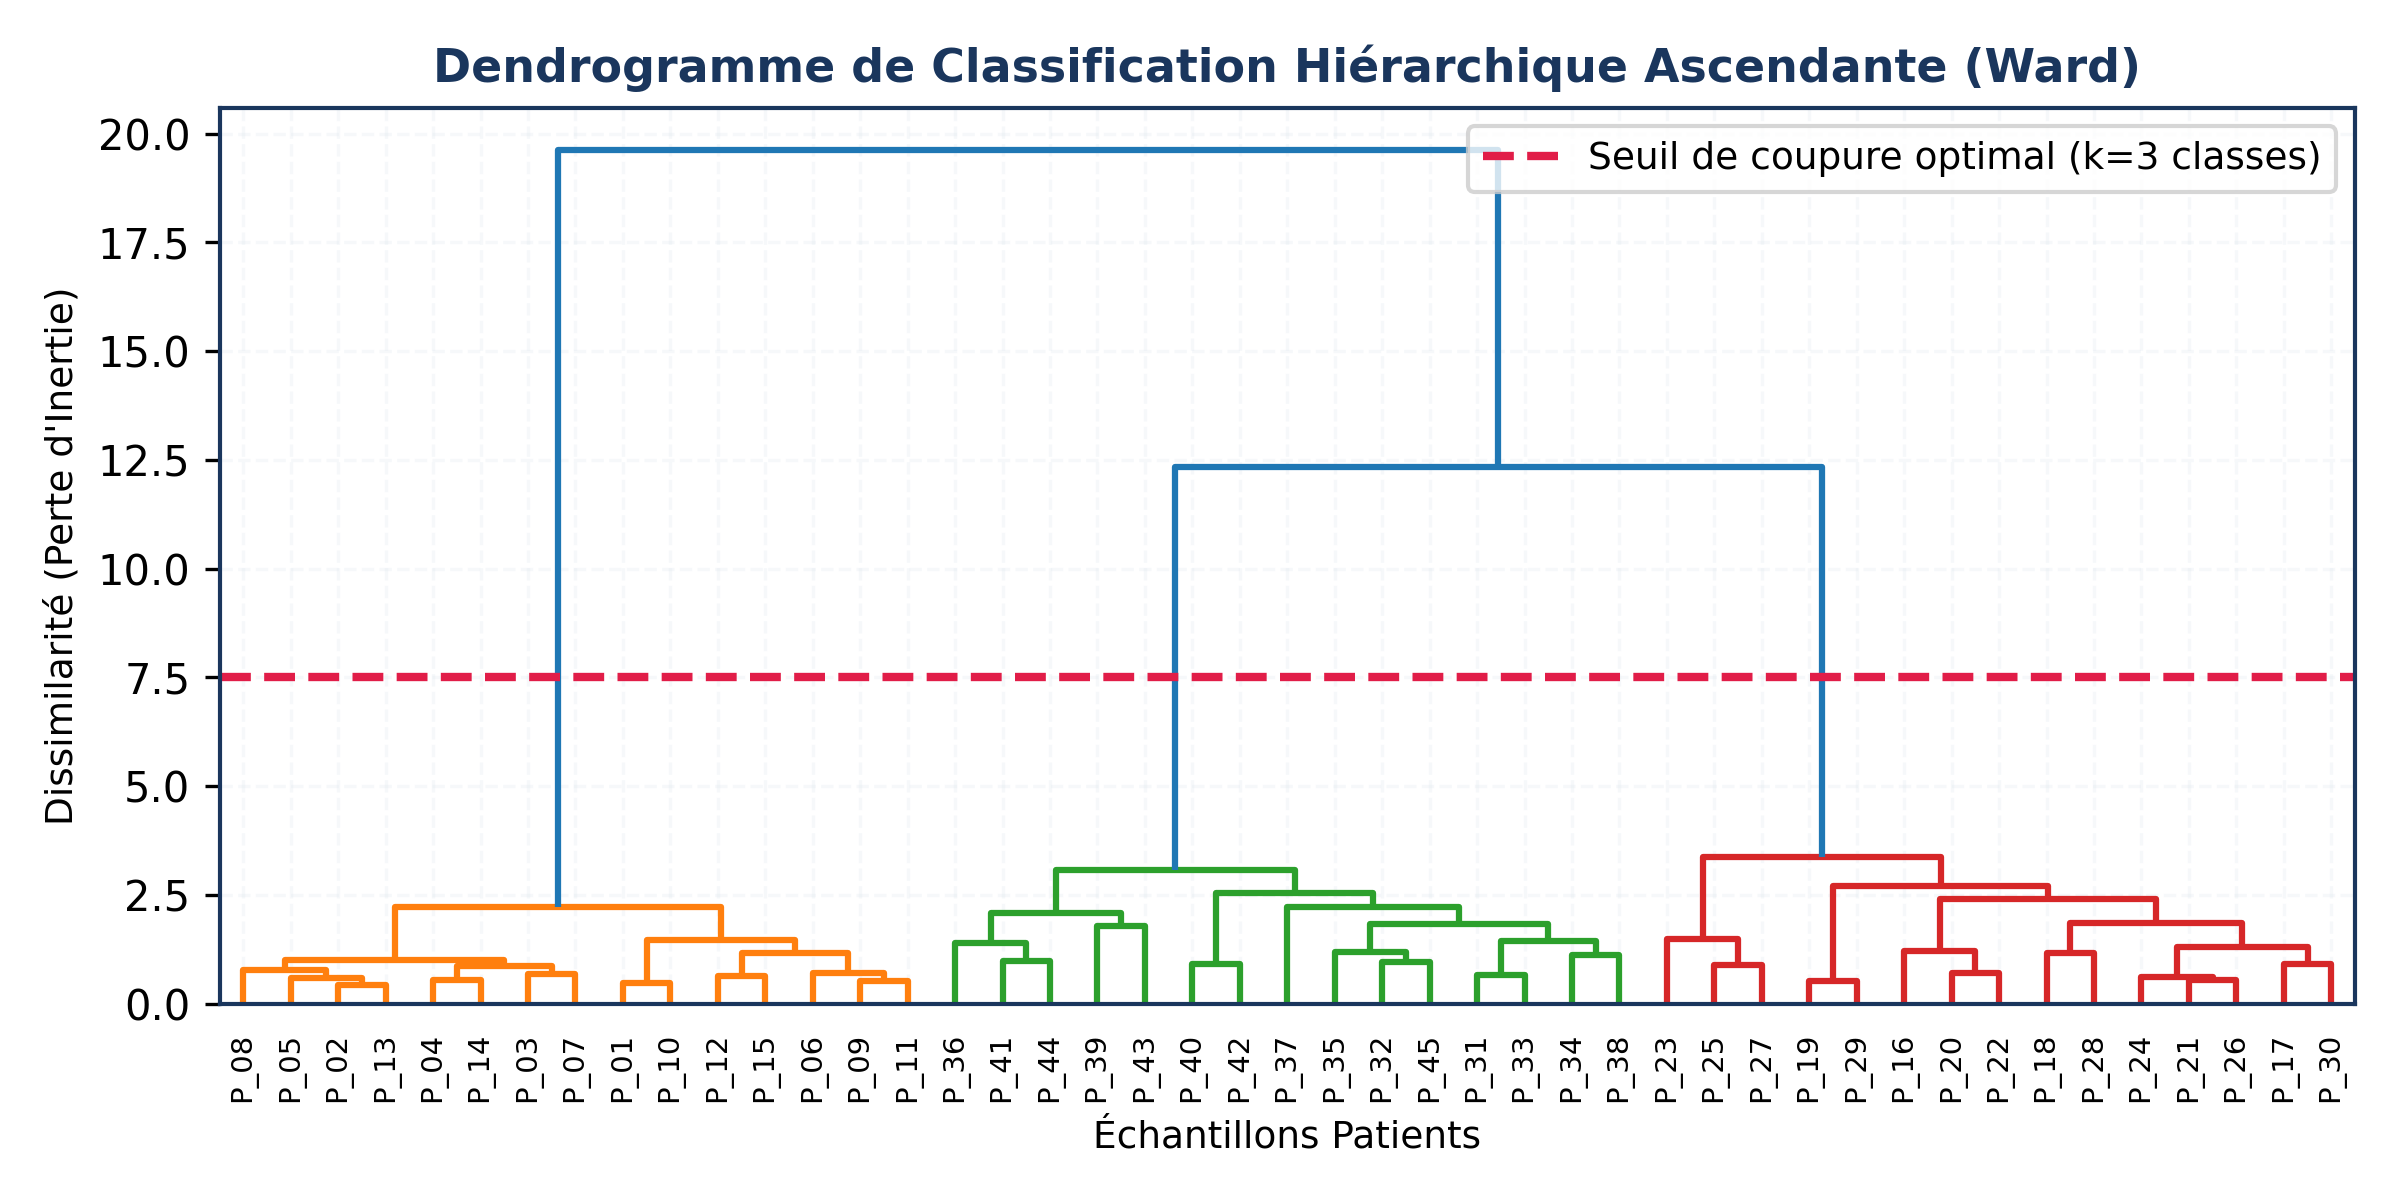
\includegraphics[height=0.48\textheight, keepaspectratio]{../figures/fig06_dendrogram_ward.png}
  \end{center}
  \vspace{-2mm}
  \begin{columns}[onlytextwidth, T]
    \begin{column}{0.48\linewidth}
      {\footnotesize \textbf{Hauteur des branches :} Représente le niveau de dissemblance entre sous-groupes fusionnés. Plus la branche verticale est longue, plus la séparation biologique est franche.}
    \end{column}
    \begin{column}{0.48\linewidth}
      {\footnotesize \textbf{Ligne de coupure horizontale :} Choisie au niveau du saut d'inertie le plus grand. Ici, le trait rouge délimite parfaitement \textbf{3 clusters cliniques distincts} ($k=3$).}
    \end{column}
  \end{columns}
\end{frame}

\begin{frame}{La Clustermap (Heatmap Bi-Clusterisée) en Biochimie}
  \begin{columns}[onlytextwidth, T]
    \begin{column}{0.48\linewidth}
      \begin{conceptbox}{Le Double Clustering Simultané}
        La Heatmap moderne croise deux CAH indépendantes :
        \begin{enumerate}
          \item \textbf{En colonnes :} Classification des biomarqueurs ou gènes (identifie les réseaux métaboliques co-activés).
          \item \textbf{En lignes :} Classification des échantillons ou patients (isole les phénotypes pathologiques).
        \end{enumerate}
      \end{conceptbox}
    \end{column}
    \begin{column}{0.48\linewidth}
      \begin{biobox}{Cas Réel : Résistance aux Antibiotiques}
        Chez 15 souches de \textit{Pseudomonas aeruginosa} testées sur 12 molécules :
        \vspace{1mm}
        \par La heatmap regroupe visuellement les souches multi-résistantes exprimant simultanément une $\beta$-lactamase à spectre étendu (BLSE) et des pompes d'efflux.
      \end{biobox}
    \end{column}
  \end{columns}
\end{frame}

\begin{frame}[plain]
  \begin{center}
    \vspace{1.8cm}
    {\Huge\color{BioNavy}\textbf{Fin du Chapitre VI}}\\[0.8cm]
    {\large Prochaine étape : Interprétation d'une Analyse Expérimentale}\\[1.2cm]
    \textbf{Dr. Sarra BENMOUMOU (Ph.D.)}\\
    \small Faculté des Sciences --- Département de Biologie\\
    \textbf{Université M'Hamed Bougara de Boumerdès (UMBB)}
  \end{center}
\end{frame}

\end{document}
